\documentclass [a4paper,11pt]{article}
\usepackage{amssymb}
\usepackage{amsthm}
\usepackage[intlimits]{amsmath}
\usepackage[polish]{babel}
\usepackage[utf8]{inputenc}
\usepackage[T1]{fontenc}
\frenchspacing
\usepackage{indentfirst}
\usepackage{graphicx}
\usepackage{subfig}
\usepackage{mathptmx}
\usepackage{geometry}
\usepackage{wrapfig}
\usepackage{enumitem}
\usepackage{tabularx}

\title{Moduł Younga}
\author{Pęcak Tomasz, Bielech Maciej}

\begin{document}
	
	\renewcommand*{\figurename}{Tabela} 
	\newgeometry{tmargin=2cm, bmargin=2cm, lmargin=2cm, rmargin=2cm}
	
	\linespread{1.5}
	\selectfont

	\begin{table}[]
		\centering
		\begin{tabular}{lllllll}
			\cline{1-6}
			\multicolumn{1}{|c|}{\begin{tabular}[c]{@{}c@{}}EAiIB\\ Informatyka\end{tabular}} & \multicolumn{2}{l|}{\begin{tabular}[c]{@{}l@{}}Pęcak Tomasz\\ Bielech Maciej\end{tabular}} & \multicolumn{1}{c|}{\begin{tabular}[c]{@{}c@{}}Rok\\ II\end{tabular}} & \multicolumn{1}{c|}{\begin{tabular}[c]{@{}c@{}}Grupa\\ 3a\end{tabular}} & \multicolumn{1}{c|}{\begin{tabular}[c]{@{}c@{}}Zespół\\ II\end{tabular}} &  \\ \cline{1-6}
			\multicolumn{1}{|c|}{\begin{tabular}[c]{@{}c@{}}Pracownia\\ FIZYCZNA\\ WFiIS AGH\end{tabular}} & \multicolumn{4}{l|}{\begin{tabular}[c]{@{}l@{}}Temat:\\ \textbf{Mostek Wheatstone'a} \end{tabular}} & 
			\multicolumn{1}{l|}{\begin{tabular}[c]{@{}l@{}}nr ćwiczenia:\\ 32\end{tabular}} &  \\ \cline{1-6}
			\multicolumn{1}{|l|}{\begin{tabular}[c]{@{}c@{}}Data wykonania:\\ 11.11.2017\end{tabular}} & \multicolumn{1}{c|}{\begin{tabular}[c]{@{}c@{}}Data oddania:\\ 14.11.2017\end{tabular}} & \multicolumn{1}{l|}{\begin{tabular}[c]{@{}l@{}}Zwrot do poprawki:\\ \phantom{data poprawki}\end{tabular}} & \multicolumn{1}{l|}{\begin{tabular}[c]{@{}l@{}}Data oddania:\\  \phantom{data oddania}\end{tabular}} & \multicolumn{1}{l|}{\begin{tabular}[c]{@{}l@{}}Data zaliczenia:\\  \phantom{data zaliczenia}\end{tabular}} & \multicolumn{1}{l|}{\begin{tabular}[c]{@{}l@{}}OCENA:\\ \phantom{ocena}\end{tabular}} &  \\ \cline{1-6} 
		\end{tabular}
	\end{table}
	 \hspace{5mm}

	\section{Wstęp}
	Celem ćwiczenia było wyznaczenie wartości modułu Younga dla stali i mosiądzu przy wykorzystaniu prawa Hooke'a.
	
	\begin{equation}
		\label{eq:prawohooka}
		\Delta l=\frac{Fl}{SE}.
	\end{equation}
	
	Moduł Younga ($E$) to współczynniki sprężystości podłużnej. Określa on własności sprężyste ciała stałego, charakteryzując podatność materiału na odkształcenia podłużne: rozciąganie, ściskanie, zgniatanie. Jego jednostką jest pascal. Możemy go obliczyć znając naprężenie $\sigma$ występujące w danym obszarze ciała oraz względne odształcenie liniowe $\epsilon$, co opisuje wzór: 
	
	\section{Wykonanie ćwiczenia}
	Ćwiczenie wykonywaliśmy dla drutów: mosiężnego i stalowego. Dla każdego z nich wykonaliśmy nastepujące czynności:
	\begin{itemize}
		\item W pierwszym kroku dokonaliśmy pomiaru długości drutu przy użyciu przymiaru milimetrowego z~dokładnością 1 mm.
		
		\item Następnie, po wcześniejszym obciążeniu drutu masą około 2kg, zmierzyliśmy średnicę drutu za pomocą śruby mikrometrycznej z~dokładnością 0,01 mm. Pomiaru tego dokonaliśmy w pięciu miejscach, aby sprawdzić czy drut ma stałą średnicę.
		
		\item Kolejnym krokiem było opróżnienie szalki z odważników i wyzerowanie czujnika mikrometrycznego.
		
		\item Po tym obciążaliśmy szalkę przez dokładanie kolejnych odważników, notując w tabeli sumaryczną masę odważników i wydłużenie drutu. Dla lepszej dokładności pomiary wykonywaliśmy przy dokładaniu odważników ($\uparrow $) i przy ich zdejmowaniu ($\downarrow $) .
		
		\item Wykonując ćwiczenie dbaliśmy o to, aby odkształcenie drutu było sprężyste, gdyż po przekroczeniu granicy sprężystości drut uległ by odkształceniu nieodwracalnemu.
		
		\item Wartosci odczytane z czujnika przenieśliśmy do tabel: (\ref{fig:tebmosiadz}, \ref{fig:tebmosiadz2}) dla mosiądzu i (\ref{fig:tabstal}) dla stali. Dla mosiądzu wykonaliśmy dwie serie pomiarów ze względu na błąd systematyczny, o który podejrzewaliśmy wyniki pierwszych pomiarów po ich wstępnej analizie.
	\renewcommand*{\figurename}{Tabela} 
	\setcounter{figure}{0}
	
	\begin{figure}[!h]
		\centering
		\caption{Pomiary oporu pierwszego rezystora}
			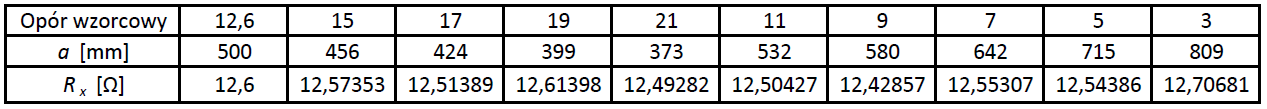
\includegraphics[width=\textwidth]{R1}
		\label{fig:r1}
	\end{figure}
	
	\begin{figure}[!h]
		\centering
		\caption{Pomiary oporu drugiego rezystora}
			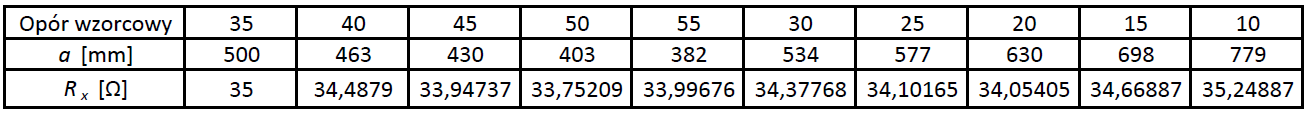
\includegraphics[width=\textwidth]{R2}
		\label{fig:r2}
	\end{figure}
	
	\begin{figure}[!h]
		\centering
		\caption{Pomiary oporu trzeciego rezystora}
		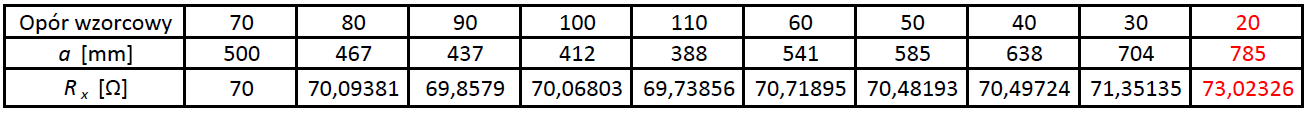
\includegraphics[width=\textwidth]{R3}
		\label{fig:r3}
	\end{figure}

	\begin{figure}[!h]
		\centering
		\caption{Pomiary oporu czwartego rezystora}
		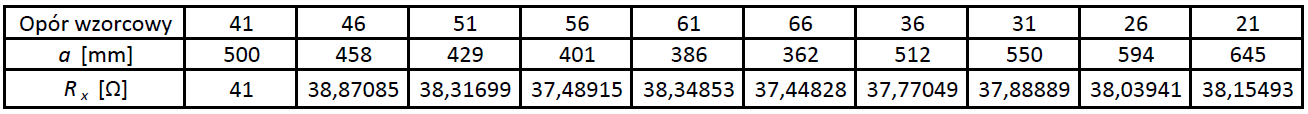
\includegraphics[width=\textwidth]{R4}
		\label{fig:r4}
	\end{figure}

	\begin{figure}[!h]
		\centering
		\caption{Pomiary oporu piątego rezystora}
		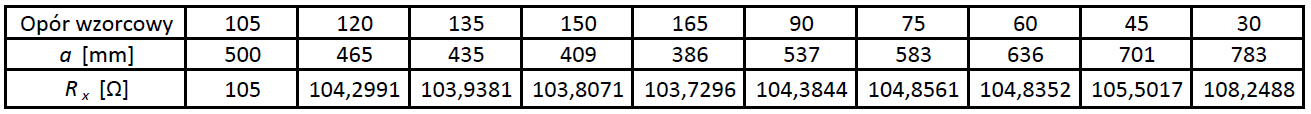
\includegraphics[width=\textwidth]{R5}
		\label{fig:r5}
	\end{figure}

	\begin{figure}[!h]
		\centering
		\caption{Pomiary oporu szeregowo podłączonych rezystorów 1 i 2}
		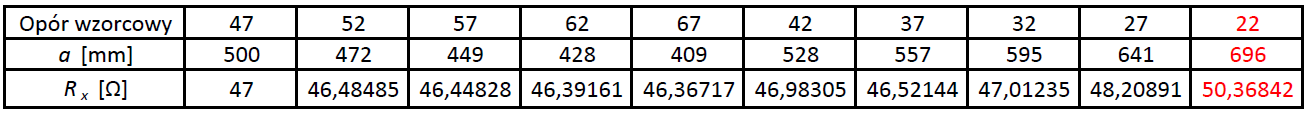
\includegraphics[width=\textwidth]{R1+R2}
		\label{fig:r1+r2}
	\end{figure}
`	
	\begin{figure}[!h]
		\centering
		\caption{Pomiary oporu równolegle podłączonych rezystorów 1 i 2}
		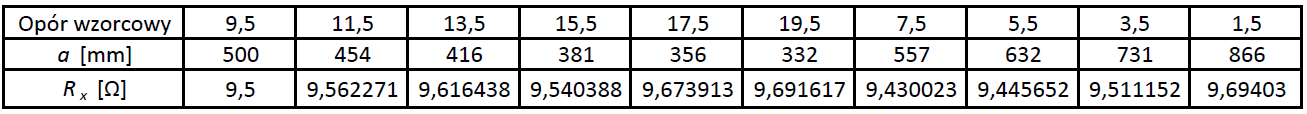
\includegraphics[width=\textwidth]{R1zR2}
		\label{fig:r1zr2}
	\end{figure}

	\begin{figure}[!h]
		\centering
		\begin{center}
		\caption{Pomiary oporu mieszanego połączenia rezystorów 1, 2 i 3}
		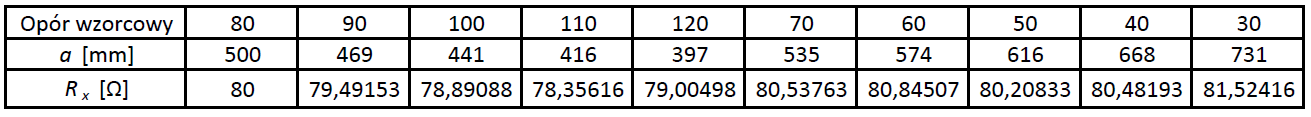
\includegraphics[width=\textwidth]{(R1zR2)+R3}
		\label{fig:(r1zr2)+r3}
		\end{center}
	\end{figure}
		
	\end{itemize}

	\renewcommand*{\figurename}{Wykres} 
	\setcounter{figure}{0}
	\newpage
	\section{Opracowanie danych pomiarowych}\label{sec:opr}
	\subsection{Pomiary i ich niepewności.}
		
		Wszystkie wielkości mierzyliśmy niewielką ilość razy, dlatego dla każdej z nich przyjmujemy ocenę niepewności typu B, co w naszym przypadku będzie odpowiadać dokładności przyrządu pomiarowego.
		\begin{enumerate}
			\item  Długość drutu: $u(l) = 1 \text{ mm}$.
			\begin{itemize}
				\item mosiężny: $ l = 1,073 \text{ m} $
				\item stalowy: $ l = 1,069 \text{ m} $
			\end{itemize}
			\item  Wydłużenie drutu: $u(\Delta l) = 0,01 \text{ mm}$.
			\item  Średnica drutu: $u(d) = 0,01 \text{ mm}$.
			\begin{itemize}
				\item mosiężny: $ d = 0,77 \text{ mm} $
				\item stalowy: $ d = 0,69 \text{ mm} $
			\end{itemize}
		\end{enumerate} 
	
	\subsection{Opracowanie danych dla drutu mosiężnego.}\label{sec:drm}
	\renewcommand*{\figurename}{Wykres} 
	\setcounter{figure}{1}
	\begin{figure}[!h]
		\centering
			%\includegraphics[width=0.8\textwidth]{wykresmosiadz1}
		\caption{Wykres zależności wydłużenia od siły dla drutu mosiężnego.}
		\label{fig:wykmosiadz}
	\end{figure}

	\begin{enumerate}[label=\alph*)]
		
		\item Analiza błędów.
		
		Nie stwierdziliśmy wystąpienia błędów grubych, gdyż na wykresie (\ref{fig:wykmosiadz}) nie zauważamy pomiarów odstających.
		
		\item Prawo przenoszenia niepewności.
		
		Wykorzystując regresję liniową, obliczamy wartość współczynnika $a$ prostej i  jej dokładność $u(a)$:
		\begin{align}
		a = 1,86 \cdot 10^{-5} \text{ }\mathrm{\frac{m}{N}},\label{a} \\
		u(a) = 3,91 \cdot 10^{-7} \text{ }\mathrm{\frac{m}{N}},
		\end{align}
		Następnie wyznaczamy moduł Younga ze wzoru roboczego (\ref{eq:wzorroboczy}).
		$$ E = 124 \text{ GPa} $$
		Obliczając niepewność złożoną (\ref{eq:niepewnosczlozonamosiadz}) oraz rozszerzoną (\ref{eq:rozszerzonamosiadz}) dochodzimy do wyników: 
		\begin{equation}
		\label{eq:niepewnosczlozonamosiadz}
		u_c(E) = \sqrt{ \left[ \frac{4}{\pi d^2a}u(l) \right]^2 + \left[ -\frac{8l}{\pi d^3 a}u(d) \right]^2 + \left[ -\frac{4l}{\pi d^2 a^2}u(a) \right]^2}
		\end{equation}
		$$ u_c(E) = 4,13 \text{ GPa,} $$
		\begin{equation}
		\label{eq:rozszerzonamosiadz}
		U(E) = k\cdot u_c(E)
		\end{equation}
		$$ U(E) = 2 \cdot 4,13 \text{ }\mathrm{GPa} = 8,26 \text{ }\mathrm{GPa} $$
		
		Niepewość względna złożona (\ref{eq:niepewnosczlozonawzglmosiadz}) jest równa:
		\begin{equation}
		\label{eq:niepewnosczlozonawzglmosiadz}
		\frac{u_c(E)}{E} = \sqrt{ \left[ \frac{u(l)}{l} \right]^2 + \left[ -2\frac{u(d)}{d} \right]^2 + \left[ -\frac{u(a)}{a} \right]^2}
		\end{equation}
		$$ \frac{u_c(E)}{E} = 3,34\% $$
		
		\item Zastosowanie niepewności rozszerzonej do oceny zgodności z wartością dokładną.
		
		Różnica pomiedzy obliczoną wartością modułu Younga ($E=123,58  \text{ }\mathrm{GPa}$), a wartością tabelaryczną wynosi:
		\begin{equation}
		\label{eq:roznicamosiadz}
		|E - E_0| = \left|124 \text{ }\mathrm{GPa} - 100 \text{ }\mathrm{GPa}\right| = 24 \text{ }\mathrm{GPa}.
		\end{equation}
		$$
		|E - E_0| > U(E)
		$$
		Wyniki pomiarów w przybliżeniu liniowe i niezgodny wynik mogą świadczyć o błędzie systematycznym. Było to złe wyzerowanie czujnika, dlatego każdy z pomiarów wskazuje niższą wartość wydłużenia drutu niż spodziewana. Błąd ten zauważyliśmy podczas wstępnej analizy pomiarów, dlatego wykonaliśmy kolejną serię pomiarów dla drutu mosiężnego.
	\end{enumerate}

	\subsection{Opracowanie danych dla drutu mosiężnego. Wyniki drugiej serii pomiarów.}
	
	\begin{figure}[!h]
		\centering
			%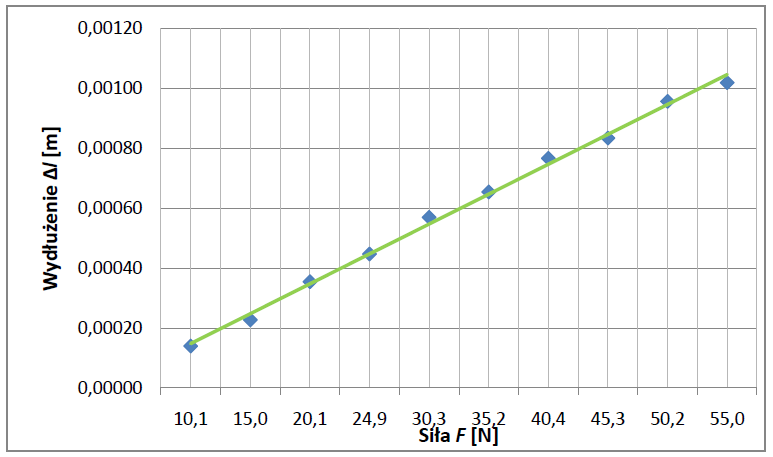
\includegraphics[width=0.8\textwidth]{wykmosiadz2}
		\caption{Wykres zależności wydłużenia od siły dla drugiej serii pomiarów drutu mosiężnego.}
		\label{fig:wykmosiadz2}
	\end{figure}
	
	\begin{enumerate}[label=\alph*)]
		\item Analiza błędów.
		
		Nie stwierdziliśmy wystąpienia błędów grubych, gdyż na wykresie (\ref{fig:wykmosiadz2}) nie zauważamy pomiarów odstających.
		
		\item Prawo przenoszenia niepewności.
		
		Analogicznie jak w podsekcji \ref{sec:drm} wyznaczamy współczynnik $a$ i wartość modułu Younga:
		\begin{align}
		a = 2,00 \cdot 10^{-5} \text{ }\mathrm{\frac{m}{N}},\label{a} \\
		u(a) = 3,50 \cdot 10^{-7} \text{ }\mathrm{\frac{m}{N}},
		\end{align}
		$$ E = 116 \text{ GPa} $$
		Obliczając niepewność złożoną (\ref{eq:niepewnosczlozonamosiadz}) oraz rozszerzoną (\ref{eq:rozszerzonamosiadz}) dochodzimy do wyników: 
		$$ u_c(E) = 3,01 \text{ GPa,} $$
		$$ U(E) = 2 \cdot 3,01 \text{ }\mathrm{GPa} = 6,02 \text{ }\mathrm{GPa} $$
		
		Niepewość względna złożona (\ref{eq:niepewnosczlozonawzglmosiadz}) jest równa:
		$$ \frac{u_c(E)}{E} = 2,6\% $$
		
		\item Zastosowanie niepewności rozszerzonej do oceny zgodności z wartością dokładną.
		
		Różnica pomiedzy obliczoną wartością modułu Younga ($E=116  \text{ }\mathrm{GPa}$), a wartością tabelaryczną wynosi:
		\begin{equation}
		\label{eq:roznicamosiadz2}
		|E - E_0| = \left|116 \text{ }\mathrm{GPa} - 100 \text{ }\mathrm{GPa}\right| = 16 \text{ }\mathrm{GPa}.
		\end{equation}
		$$
		|E - E_0| > U(E)
		$$
		
		
	\end{enumerate}

	\subsection{Opracowanie danych dla drutu stalowego.}
	\begin{figure}[!h]
		\centering
			%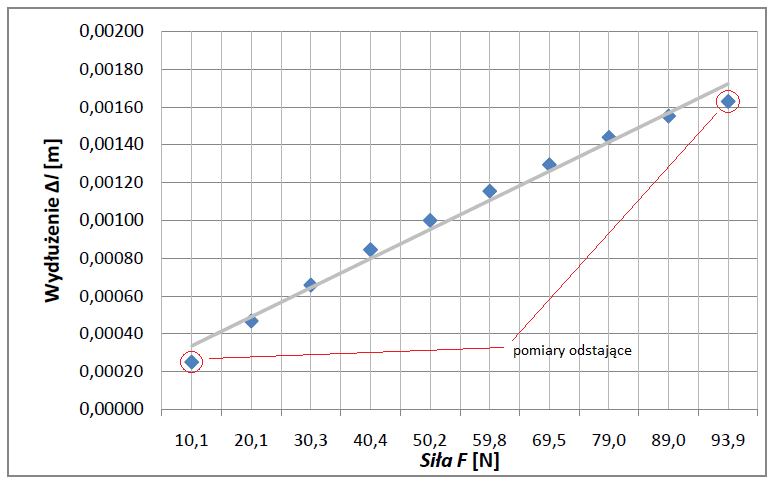
\includegraphics[width=0.8\textwidth]{wykstal}
		\caption{Wykres zależności wydłużenia od siły dla drutu stalowego.}
		\label{fig:wykstal}
	\end{figure}
	
	\begin{enumerate}[label=\alph*)]
		\item Analiza błędów.
		
		Stwierdziliśmy wystąpienie dwóch pomiarów odstających, które możemy utożsamiać z błędami grubymi. Błędy te zaznaczylismy na wykresie (\ref{fig:wykstal}). Mogły one zostać spowodowane niewystarczającym wydłużeniem dla pierwszego pomiaru, a dla ostatniego pomiaru zbyt dużym naprężeniem, zbliżonym do granicy sprężystości, lub błędnym odczytem pomiaru z czujnika.
		
		\item Prawo przenoszenia niepewności.
		
		Podobnie jak dla drutu mosiężnego w podsekcji \ref{sec:drm} wyznaczamy współczynnik $a$ i wartość modułu Younga:
		\begin{align}
		a = 1,60 \cdot 10^{-5} \text{ }\mathrm{\frac{m}{N}},\label{a} \\
		u(a) = 4,55 \cdot 10^{-7} \text{ }\mathrm{\frac{m}{N}},
		\end{align}
		$$ E = 176 \text{ GPa} $$
		Obliczając niepewność złożoną (\ref{eq:niepewnosczlozonamosiadz}) oraz rozszerzoną (\ref{eq:rozszerzonamosiadz}) dochodzimy do wyników: 
		$$ u_c(E) = 7,13 \text{ GPa,} $$
		$$ U(E) = 2 \cdot 7,13 \text{ }\mathrm{GPa} = 14,26 \text{ }\mathrm{GPa} $$
		
		Niepewość względna złożona jest równa:
		$$ \frac{u_c(E)}{E} = 4,03\% $$
		
		\item Zastosowanie niepewności rozszerzonej do oceny zgodności z wartością dokładną.
		
		Różnica pomiedzy obliczoną wartością modułu Younga ($E=176,47  \text{ }\mathrm{GPa}$), a wartością tabelaryczną wynosi:
		\begin{equation}
		\label{eq:roznicastal}
		|E - E_0| = \left|176 \text{ }\mathrm{GPa} - 215 \text{ }\mathrm{GPa}\right| = 39 \text{ }\mathrm{GPa}.
		\end{equation}
		$$
		|E - E_0| > U(E)
		$$	
	\end{enumerate}
	
	\section{Podsumowanie}
	\begin{center}
		\begin{tabular}{|c|c|c|c|c|c|c|}
			\hline Opis wielkości & $ E_0 \left[ \text{GPa} \right]$ & $E \left[ \text{GPa} \right]$ & $U(E) \left[ \text{GPa} \right]$ & $ \frac{u(E)}{E} $& $(0,9E_0-U(E); 1,1E_0 + U(E))$\\
			\hline Pomiary drutu mosiężnego I & 100 & 124 & 8 & 3,34 \% & (82 ;118) \\
			\hline Pomiary drutu mosiężnego II & 100 & 116 & 6 & 2,6 \% & (84 ; 116) \\  
			\hline Pomiary drutu stalowego & 210-220 & 176  & 14 &  4,03 \% & (175 ; 256)\\ 
			\hline 
		\end{tabular} 
	\end{center}
\vspace{1em}

\begin{itemize}
	\item Określenie poprawności wyników naszych doświadczeń jest trudne, ponieważ nie da się jednoznacznie określić wartości tabelarycznej dla danego metalu. Wynika to z nieznajomości dokładnego składu metalu (stopu), a także ze zużycia drutu. W naszych badaniach przyjmujemy rozrzut rzędu $\pm10\%$ dla wartości odczytanych z tabel fizycznych.
	
	\item Zarówno dla pierwszych jak i drugich pomiarów dla mosiądzu obliczona wartość modułu wykracza poza przedział ($E_0-U(E), E_0+U(E)$). Po uwzględnieniu dziesięcioprocentowego rozrzutu drugą serię pomiarów możemy uznać za poprawną w zakresie wyznaczonej niepewności. Pierwsza seria pomiarów nadal daje wynik niepoprawny, co potwierdza nasze obawy co do błędu systematycznego.
	
	\item Podobnie jak w przypadku drugiej serii pomiarów dla mosiądzu wartość modułu Younga dla stali wykracza poza $E_0 \pm U(E)$, lecz po uwzględnieniu dziesięcioprocentowego rozrzutu od wartości tablicowej możemy uznać obliczoną wartość za poprawną w zakresie wyznaczonej niepewności.
\end{itemize}

\end{document}